%%%%%%%%%%%%%%%%%%%%%%%%%% lecture-1
\begin{frame}
  \frametitle{lecture-3 主要内容}
  \framesubtitle{最简单的C语言程序设计---顺序程序设计}
  \tableofcontents[hideallsubsections]
\end{frame}

\section{初识C语言程序(讲解作业)}

\begin{frame}[fragile]{DevC++ 5.0以前的版本}
\begin{lstlisting}
#include<stdio.h>            // standard input/output编译预处理指令
#include <stdlib.h>          // standard library function, eg. for system()函数 
int main()                   // 主函数
{                            // 函数开始标志
   printf("%d\n",p);
   system(“pause”);          // 窗口暂停,DevC++ 5.0以前的版本。[机试系统提交时,一定注释或删除该语句] 
   return 0;                 // 函数执行完毕返回函数值0
}                            // 函数结束标志
\end{lstlisting}
\end{frame}

\begin{frame}[fragile]{求5!的C语言程序}
\begin{lstlisting}
#include<stdio.h>            // standard input/output编译预处理指令
int main()                   // 主函数
{                            // 函数开始标志
   int i,p;  // p表示被乘数, i表示乘数
   p=1;
   i=2;
   while(i<=5)
   {  
      p=p*i;
      i++; // i = i + 1
   }
   printf("%d\n",p);
   return 0;                 // 函数执行完毕返回函数值0
}                            // 函数结束标志
\end{lstlisting}
\end{frame}

\begin{frame}[fragile]{变量在使用之前首先要定义它的数据类型}
\begin{lstlisting}
#include<stdio.h>            // standard input/output编译预处理指令
int main()                   // 主函数
{                            // 函数开始标志
   int a,b;  // 定义变量a, b为整型数值,同类型变量可以在一条语句中定义。
   float f;  // 定义变量f为单精度浮点数
   double d; // 定义变量d为双精度浮点数
   char c;   // 定义变量c为单个英文字母
   a=10;
   b=20;
   f=10.2;
   d=20.3;
   c='A';
   return 0;                 // 函数执行完毕返回函数值0
}                            // 函数结束标志
\end{lstlisting}
\end{frame}

\begin{frame}[fragile]{if(条件表达式)\{ 表达式为真(非0)时执行语句; \}}
\begin{lstlisting}
#include<stdio.h>            // standard input/output编译预处理指令
int main()                   // 主函数
{                            // 函数开始标志
   int a=10;    // 定义变量a为整型数值, 定义变量时,可以指定变量的初值
   if(a>=10)
   {
      printf("a>=10\n"); // \n为换行符
   }
   else
   {
      printf("a<10\n"); // \n为换行符
   }
   return 0;                 // 函数执行完毕返回函数值0
}                            // 函数结束标志
\end{lstlisting}
\end{frame}

\begin{frame}[fragile]{while(条件表达式)\{ 表达式为真(非0)时执行的语句;\}}
\begin{lstlisting}
#include<stdio.h>            // standard input/output编译预处理指令
int main()                   // 主函数
{                            // 函数开始标志
   int a=10;    // 定义变量a为整型数值, 定义变量时,可以指定变量的初值
   while(a>=0)
   {
     printf("a=%d\n",a); // \n为换行符
     a--; // a= a - 1
   }
   return 0;                 // 函数执行完毕返回函数值0
}                            // 函数结束标志
\end{lstlisting}
\end{frame}

\section{数据的输入输出}

\begin{frame}{常用格式描述符与数据类型的对应关系}
\begin{tabular}{|c|c|c|}
	\hline 
	\textbf{格式符} & \textbf{对应的数据类型} &  \textbf{备注}\\ 
	\hline 
	\%d & int &  \\ 
	\hline  
	\%f & float &  \\
	\hline
	\%c & char & \\ 
	\hline   
	\%lf & double & \\ 
	\hline 
	\%.2f & float & 保留两位小数, 四舍五入。不适用于scanf()。 \\ 
	\hline 
	\%.2lf & double & 保留两位小数, 四舍五入。不适用于scanf()。 \\ 
	\hline
	\hline   
	\%x & int & 十六进制显示 \\ 
	\hline 
	\%ld & long int &  \\ 
	\hline 
\end{tabular}
\newline
\newline
\textcolor{blue}{详见p73, 表3.6}
\end{frame}

\begin{frame}[shrink,fragile]{输出语句printf(``原样输出, \%格式符'', 对应变量值);}
\begin{lstlisting}
#include<stdio.h>            // standard input/output编译预处理指令
int main()                   // 主函数
{                            // 函数开始标志
   int a=10,b;    // 定义变量a, b为整型数值, 定义变量时,可以指定变量的初值
   float f=10.2;  // 定义变量f为单精度浮点数
   double d; // 定义变量d为双精度浮点数
   char c;   // 定义变量c为单个英文字母
   f=10.2;
   d=20.356;
   c='A';
   printf("a=%d,b=%d,c=%c,f=%f,d=%.2lf\n",a,b,c,f,d); // %.2f, %.2lf保留两位小数
   return 0;                 // 函数执行完毕返回函数值0
}                            // 函数结束标志
\end{lstlisting}
\textcolor{blue}{变量b没有被赋值, 将是一个随机值。}
\end{frame}

\begin{frame}[fragile]{输入语句scanf(``\%变量格式符'', \&变量名);}
\begin{lstlisting}
#include<stdio.h>            // standard input/output编译预处理指令
int main()                   // 主函数
{                            // 函数开始标志
   int a=10,b;    // 定义变量a, b为整型数值, 定义变量时,可以指定变量的初值
   float f=10.2;  // 定义变量f为单精度浮点数
   double d; // 定义变量d为双精度浮点数
   char c='A';   // 定义变量c为单个英文字母, 字符输入以后讲
   printf("请输入整数和浮点数, 空格隔开:\n"); // 提示语句[可选]
   scanf("%d%f",&a,&f);  // 尽量简单, 不要有其它字符和'\n'
   printf("请输入两个浮点数, 空格隔开:\n"); // 提示语句[可选]
   scanf("%f%lf",&f,&d);
   printf("a=%d,b=%d,c=%c,f=%f,d=%lf\n",a,b,c,f,d); // \n为换行符
   return 0;                 // 函数执行完毕返回函数值0
}                            // 函数结束标志
\end{lstlisting}
\end{frame}

\begin{frame}[fragile]{字符输出函数putchar}
\begin{lstlisting}
#include<stdio.h>
int main()
{
   char a = 'B',b = 'O',c = 'Y'; //定义3个字符变量并初始化
   putchar(a); //向显示器输出字符B
   putchar(b); //向显示器输出字符O
   putchar(c); //向显示器输出字符Y
   putchar ('\n'); //向显示器输出一个换行符
   return 0;
}
\end{lstlisting}
\end{frame}

\begin{frame}[fragile]{字符输入函数getchar, 遇到回车, 开始从缓冲区中接收字符。}
\begin{lstlisting}
#include<stdio.h>
int main()
{
   char a,b,c;  //定义字符变量a,b,c
   a = getchar();  //从键盘输入一个字符,送给字符变量a
   b = getchar();  //从键盘输入一个字符,送给字符变量b
   c = getchar();  //从键盘输入一个字符,送给字符变量c
   putchar(a);  //将变量a的值输出
   putchar(b);  //将变量b的值输出 
   putchar(c);  //将变量c的值输出
   printf("\na=%d,b=%d,c=%d,a=%c,b=%c,c=%c\n",a,b,c,a,b,c);
   return 0;
}
\end{lstlisting}
\end{frame}

\begin{frame}[fragile]{字符输入函数getchar, 遇到回车, 开始从缓冲区中接收字符。}
\begin{lstlisting}
char a,b,c;  //定义字符变量a,b,c
a = getchar();  //从键盘输入一个字符,送给字符变量a
b = getchar();  //从键盘输入一个字符,送给字符变量b
c = getchar();  //从键盘输入一个字符,送给字符变量c
putchar(a);  //将变量a的值输出
putchar(b);  //将变量b的值输出 
putchar(c);  //将变量c的值输出
printf("\na=%d,b=%d,c=%d,a=%c,b=%c,c=%c\n",a,b,c,a,b,c);
\end{lstlisting}
从键盘输入abc回车, 观察结果, 应该是正确的结果。
遇到回车, 开始从缓冲区中接收字符。
\end{frame}

\begin{frame}[fragile]{字符输入函数getchar, 遇到回车, 开始从缓冲区中接收字符。}
\begin{lstlisting}
a = getchar();  //从键盘输入一个字符,送给字符变量a
b = getchar();  //从键盘输入一个字符,送给字符变量\n
c = getchar();  //从键盘输入一个字符,送给字符变量b
putchar(a);  //将变量a的值输出a
putchar(b);  //将变量b的值输出\n 
putchar(c);  //将变量c的值输出b
printf("\na=%d,b=%d,c=%d,a=%c,b=%c,c=%c\n",a,b,c,a,b,c);
\end{lstlisting}
再运行一次程序, 输入a回车, 输入b回车, 输入c回车, 观察结果。\\
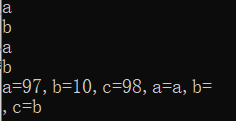
\includegraphics[scale=0.5]{abc}
\end{frame}

\begin{frame}
根据学生的反馈,数据的输入语句没有完全听明白。 \\
下一讲, 进一步详细讲解。\\
欢迎同学们在群里踊跃发言,任何不理解的知识点请指出来,我将在以后的讲课中,有针对性的讲清楚大家有疑惑的问题。一些与编程无关的俏皮话之类的东西就不要发了,争取把我们这个群建立成纯净的,对大家学习课程有帮助的程序设计讨论群。力争100名学生一个都不掉队,考个好成绩。加油!!
\end{frame}



